


% \draft{In the last chapter, we summarized how the visibilities were calibrated by ALMA before we recieved the data. Beause IRS 63 is a bright and nearby source the observations have a high SNR, sllowing us to do self-calibration. Self-calibration is useful to get rid of the `stuff' that pops up but is not really there, called an artifact \citep{Marvil2}. First, there could be artifacts from the srouce duue to calibration errors such as differences in the astmosphere over each dish \citep{Marvil2}. Secondly, there could be artifacts from a backgrournd source due to direction-independent calibration errors, such as antenna based gain changes \citep{Marvil2}.}


In this section, the self-calibration details for this project are summarized. The data at \bfourNS, \bfive and \bseven were calibrated as part of this project, and the \bsix data were provided from \cite{sadavoy_dust_2019}.


To clean the data,  \texttt{tclean} was used in Common Astronomy Software Applications (CASA) version 5.6.1-8 \SCC{add casa citation}. The images were cleaned using the multi-scale multi-frequency deconvolution algorithm (MS-MFS, \texttt{deconvolver = `mtmfs'}). Different values of nterms were explored and no significant change between \texttt{nterms = 1} and nterms = 2 were found. The images presented in this thesis have nterms = 2 for \bfour and \bsevenNS, nterms = 1 for \bfive and \bsixNS. 
\question{band 5 nterms = ?} The Briggs weighting scheme was used with \texttt{robust = 0.5} for all wavleengths except the \bfive data where w\texttt{robust = -1} was used to better match the resolution of the other datasets (see Chapter \ref{sec: discussion_band5_data_issues} for more details). 



The \SI images at each band had an interactive clean at both phase and amplitude calibration. We began with a shallow phase calibration, and progressively cleaned deeper each time for a total of three rounds. Then, two rounds of amplitude and phase self calibration. \SC{Add more info.} Additionally, the \SQ and \SU data were also cleaned using a non-interactive phase calibration using the final mask from the amplitude calibration at its respective wavelength.  \SC{Add more info}


Below, in Figure \ref{fig: BeforeAndAfterClean}, is an example of IRS 63 at \bfour before and after self calibration. We can see how cleaning the image removed background noise. The \SNR values also improved, going from 660 to 2655. \question{Report the S/N change for the other bands?}. The final self-calibrated \SI maps produced using this method are presented in Chapter \ref{sec: chap4_stokesI}.


\SC{It may be worth here or in the previous section to explain how self-calibration can improve the S/N.}



\begin{figure}[h]
  \centering
  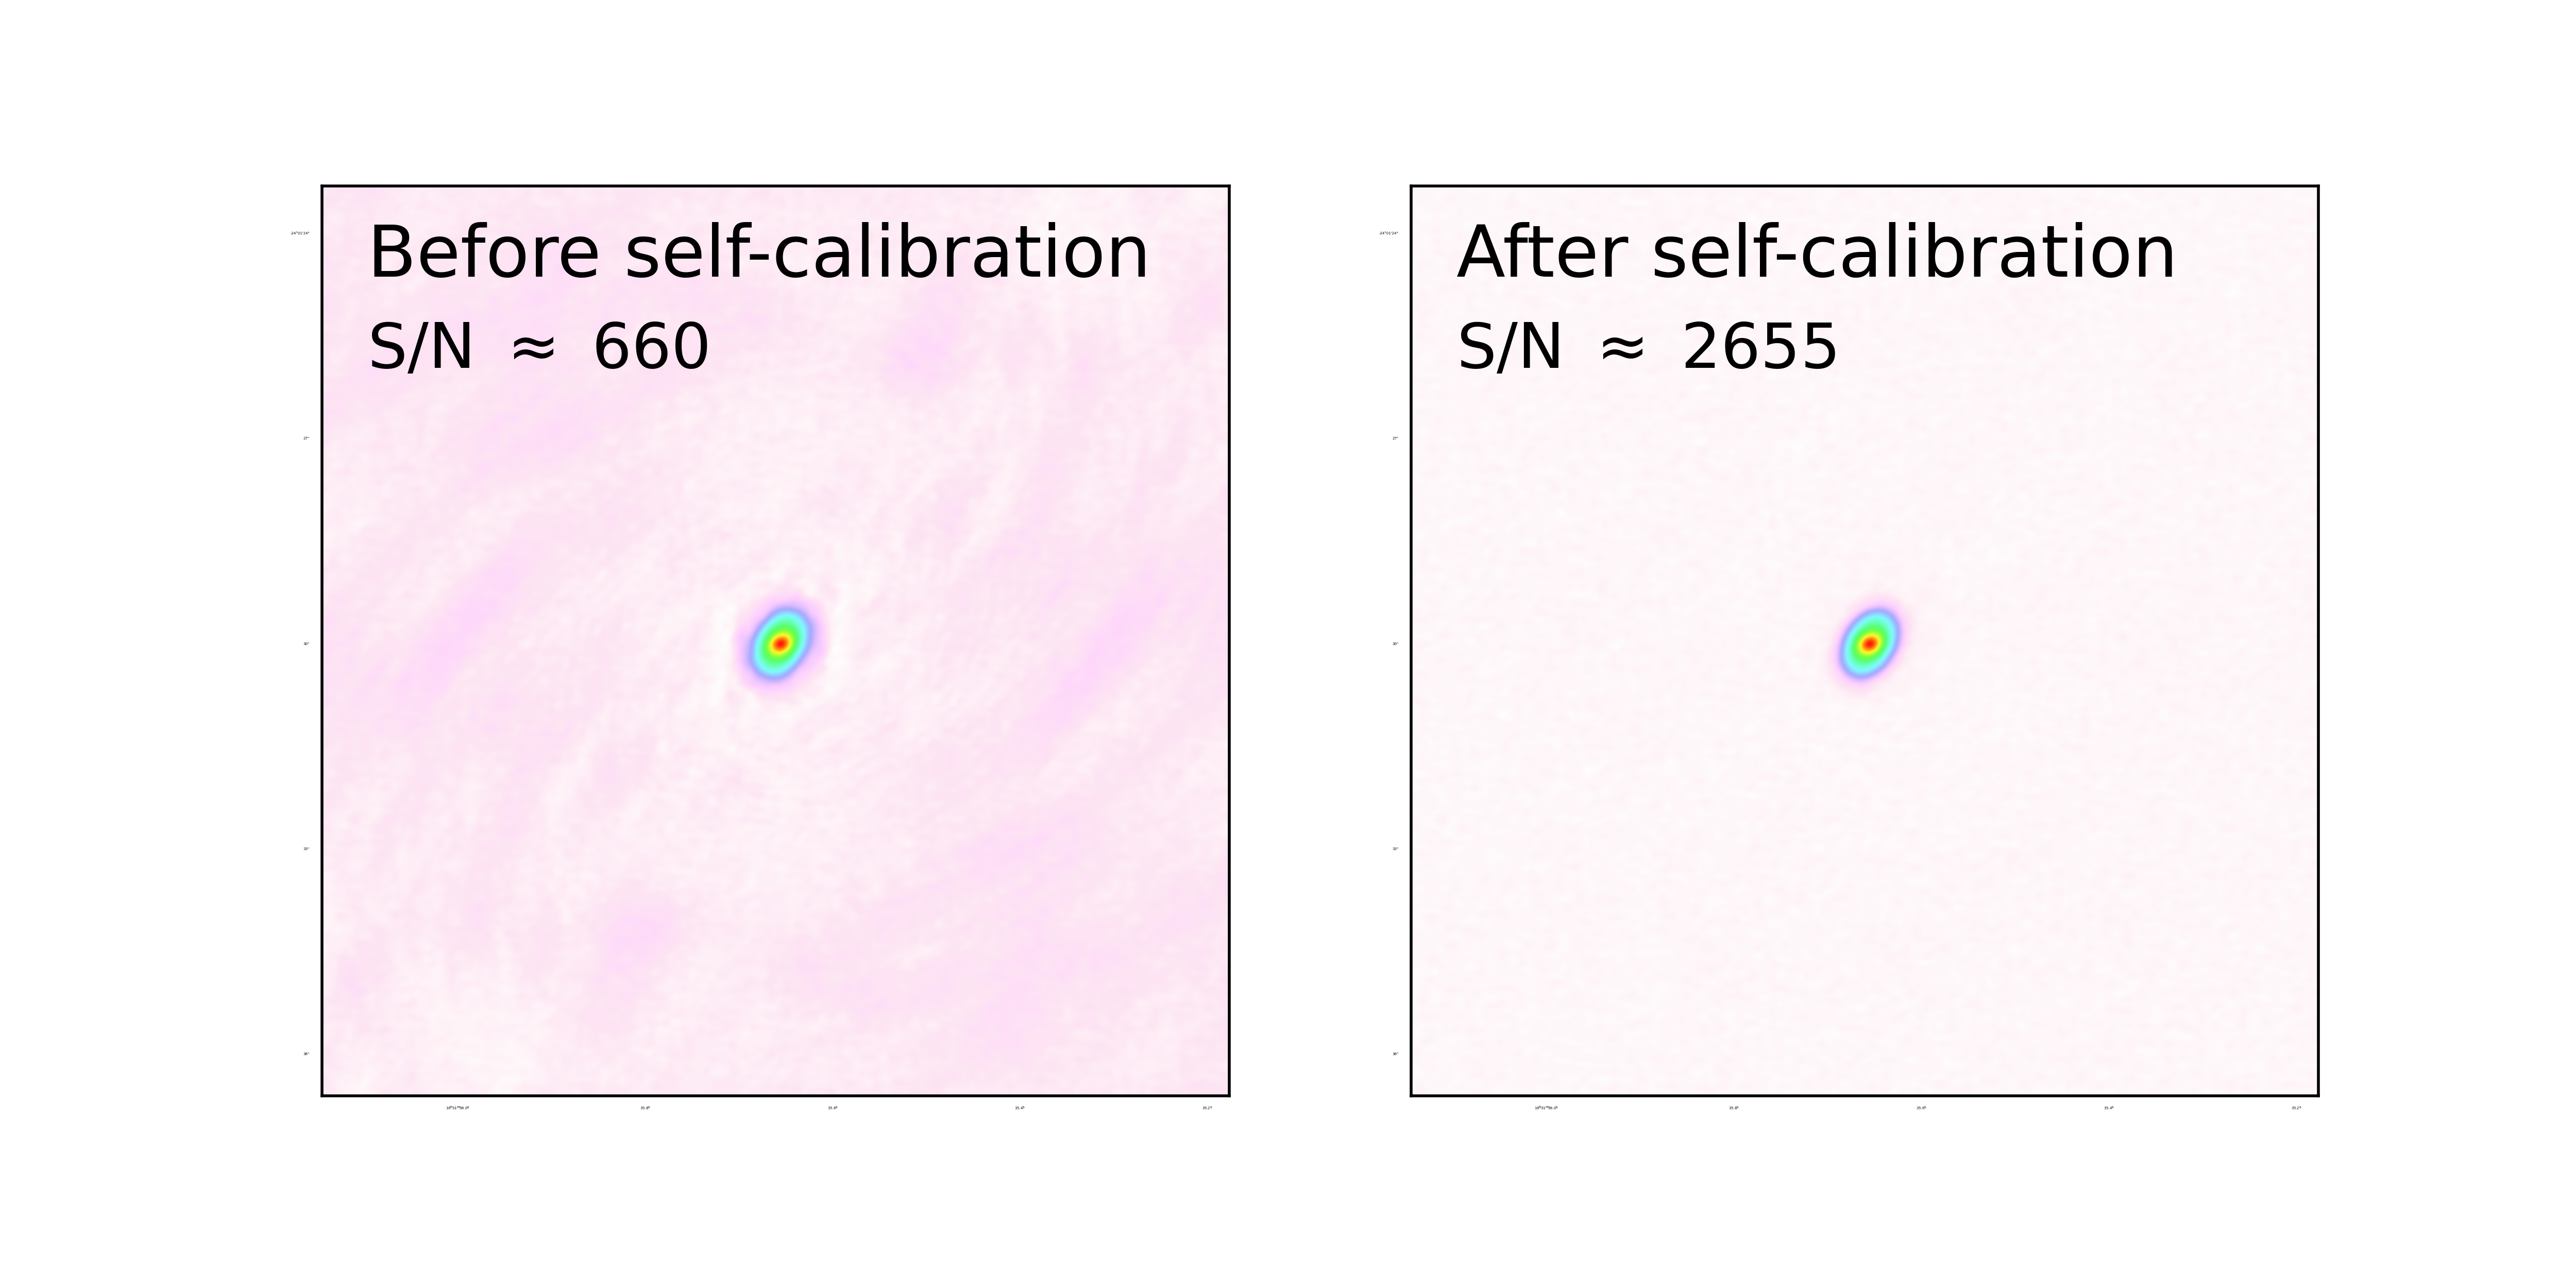
\includegraphics[width=1.25\textwidth]{WRITEUP_AND_IMAGES/IMAGES/WRITEUP/BeforeAndAfterClean.png}
  \caption{Images before (left) and after (right) self-calibration at \bfour. Images shown to demonstrate how background noise is reduced the self-calibration process, and improved the peak \SNRns.}
  \label{fig: BeforeAndAfterClean}
\end{figure}




\SCC{The results of the self-cleaning process are presented in Table \ref{tab: source_info}, including the synthesized beam size, reported as major and minor axes and position angle. } Additionally, the centre position of the disk in Right Ascension (RA) and Declination (Dec) and the position angle of the disk found using \SCC{\texttt{imfit} in CASA.}


\begin{table}[h!]
\centering
\caption{Summary of properties of the cleaned images of IRS 63. \add{Band 5 robust -1 not 0.5, nterms and robust}}
\begin{tabular}{lcccc}
\toprule
\textbf{Property} & \textbf{\bandfourmm} & \textbf{\bandfivemm } & \textbf{\bandsixmm } & \textbf{\bandsevenmm} \\
\midrule


R.A. (h, m, s) 
& 16:31:35.656 
& 16:31:35.656 \note{check}
& 16:31:35.657  
& 16:31:35.656 \\

Decl. (J2000) 
& -24:01:29.992 
& -24:01:30.086 \note{check}
& -24:01:29.935 
& -24:01:30.089 \\


Beam ($''\times''$) 
& 0.18 $\times$ 0.13 
& 0.23 $\times$ 0.18 
& 0.27 $\times$ 0.20 
& 0.28 $\times$ 0.17 \\



Beam PA ($^\circ$) 
& -81.0 
& -88.9 \add{$\Delta$ to rob-1}
& -68.6
& -81.2 \\


Disk PA ($^\circ$) 
& 145.9 
& 148.39 \note{check}
& 148.0 
& 139.7 \\

\texttt{nterms}
& \add{num}
& \add{num}
& \add{num} 
& \add{num} \\

\texttt{robust}
& \add{num}
& \add{num}
& \add{num} 
& \add{num} \\



\bottomrule
\end{tabular}
\label{tab: source_info}
\end{table}




% ---------------------------------------------

